\section{Introduction}
The formation of carbonaceous nanoparticles such as soot and Carbon Black (CB) is a complex, multiscale process involving chemical reactions, heat transfer, fluid dynamics, and particle dynamics, and spans wide spatial ($\sim 10^{-9}$ to 1~m) and temporal ($\sim 10^{-10}$ to 1~s) scales. Figure~\ref{fig:sootscales} illustrates the length and time scales relevant to different stages of soot formation, from PAH precursors to incipient, nascent, and mature soot in flames. Understanding the effect of process parameters on the morphology and composition of carbonaceous nanoparticles is crucial to assess the health and environmental impacts of soot and the functional properties of CB.


Soot is a broadband light absorber~\cite{d2009combustion} and is emitted on a large scale ($\sim 9.5$~megatons per year~\citep{myhre2014anthropogenic}), making it the third strongest contributor to climate change after methane and carbon dioxide. Its fine particulate nature ($\mathrm{PM_{2.5}}$) also poses serious health risks~\citep{borm2004inhaled}. In contrast, CB is the largest flame-made nanomaterial by production volume ($\sim15$~megatons annually~\citep{rosner2024techno}) and plays a vital role in industrial applications, including rubber reinforcement~\citep{international2016carbon} and lithium-ion batteries~\citep{Palomares2010}.




\begin{figure}[H]
	\centering
	\begin{tikzpicture}
		\draw (0, 0) node[inner sep=0] 	{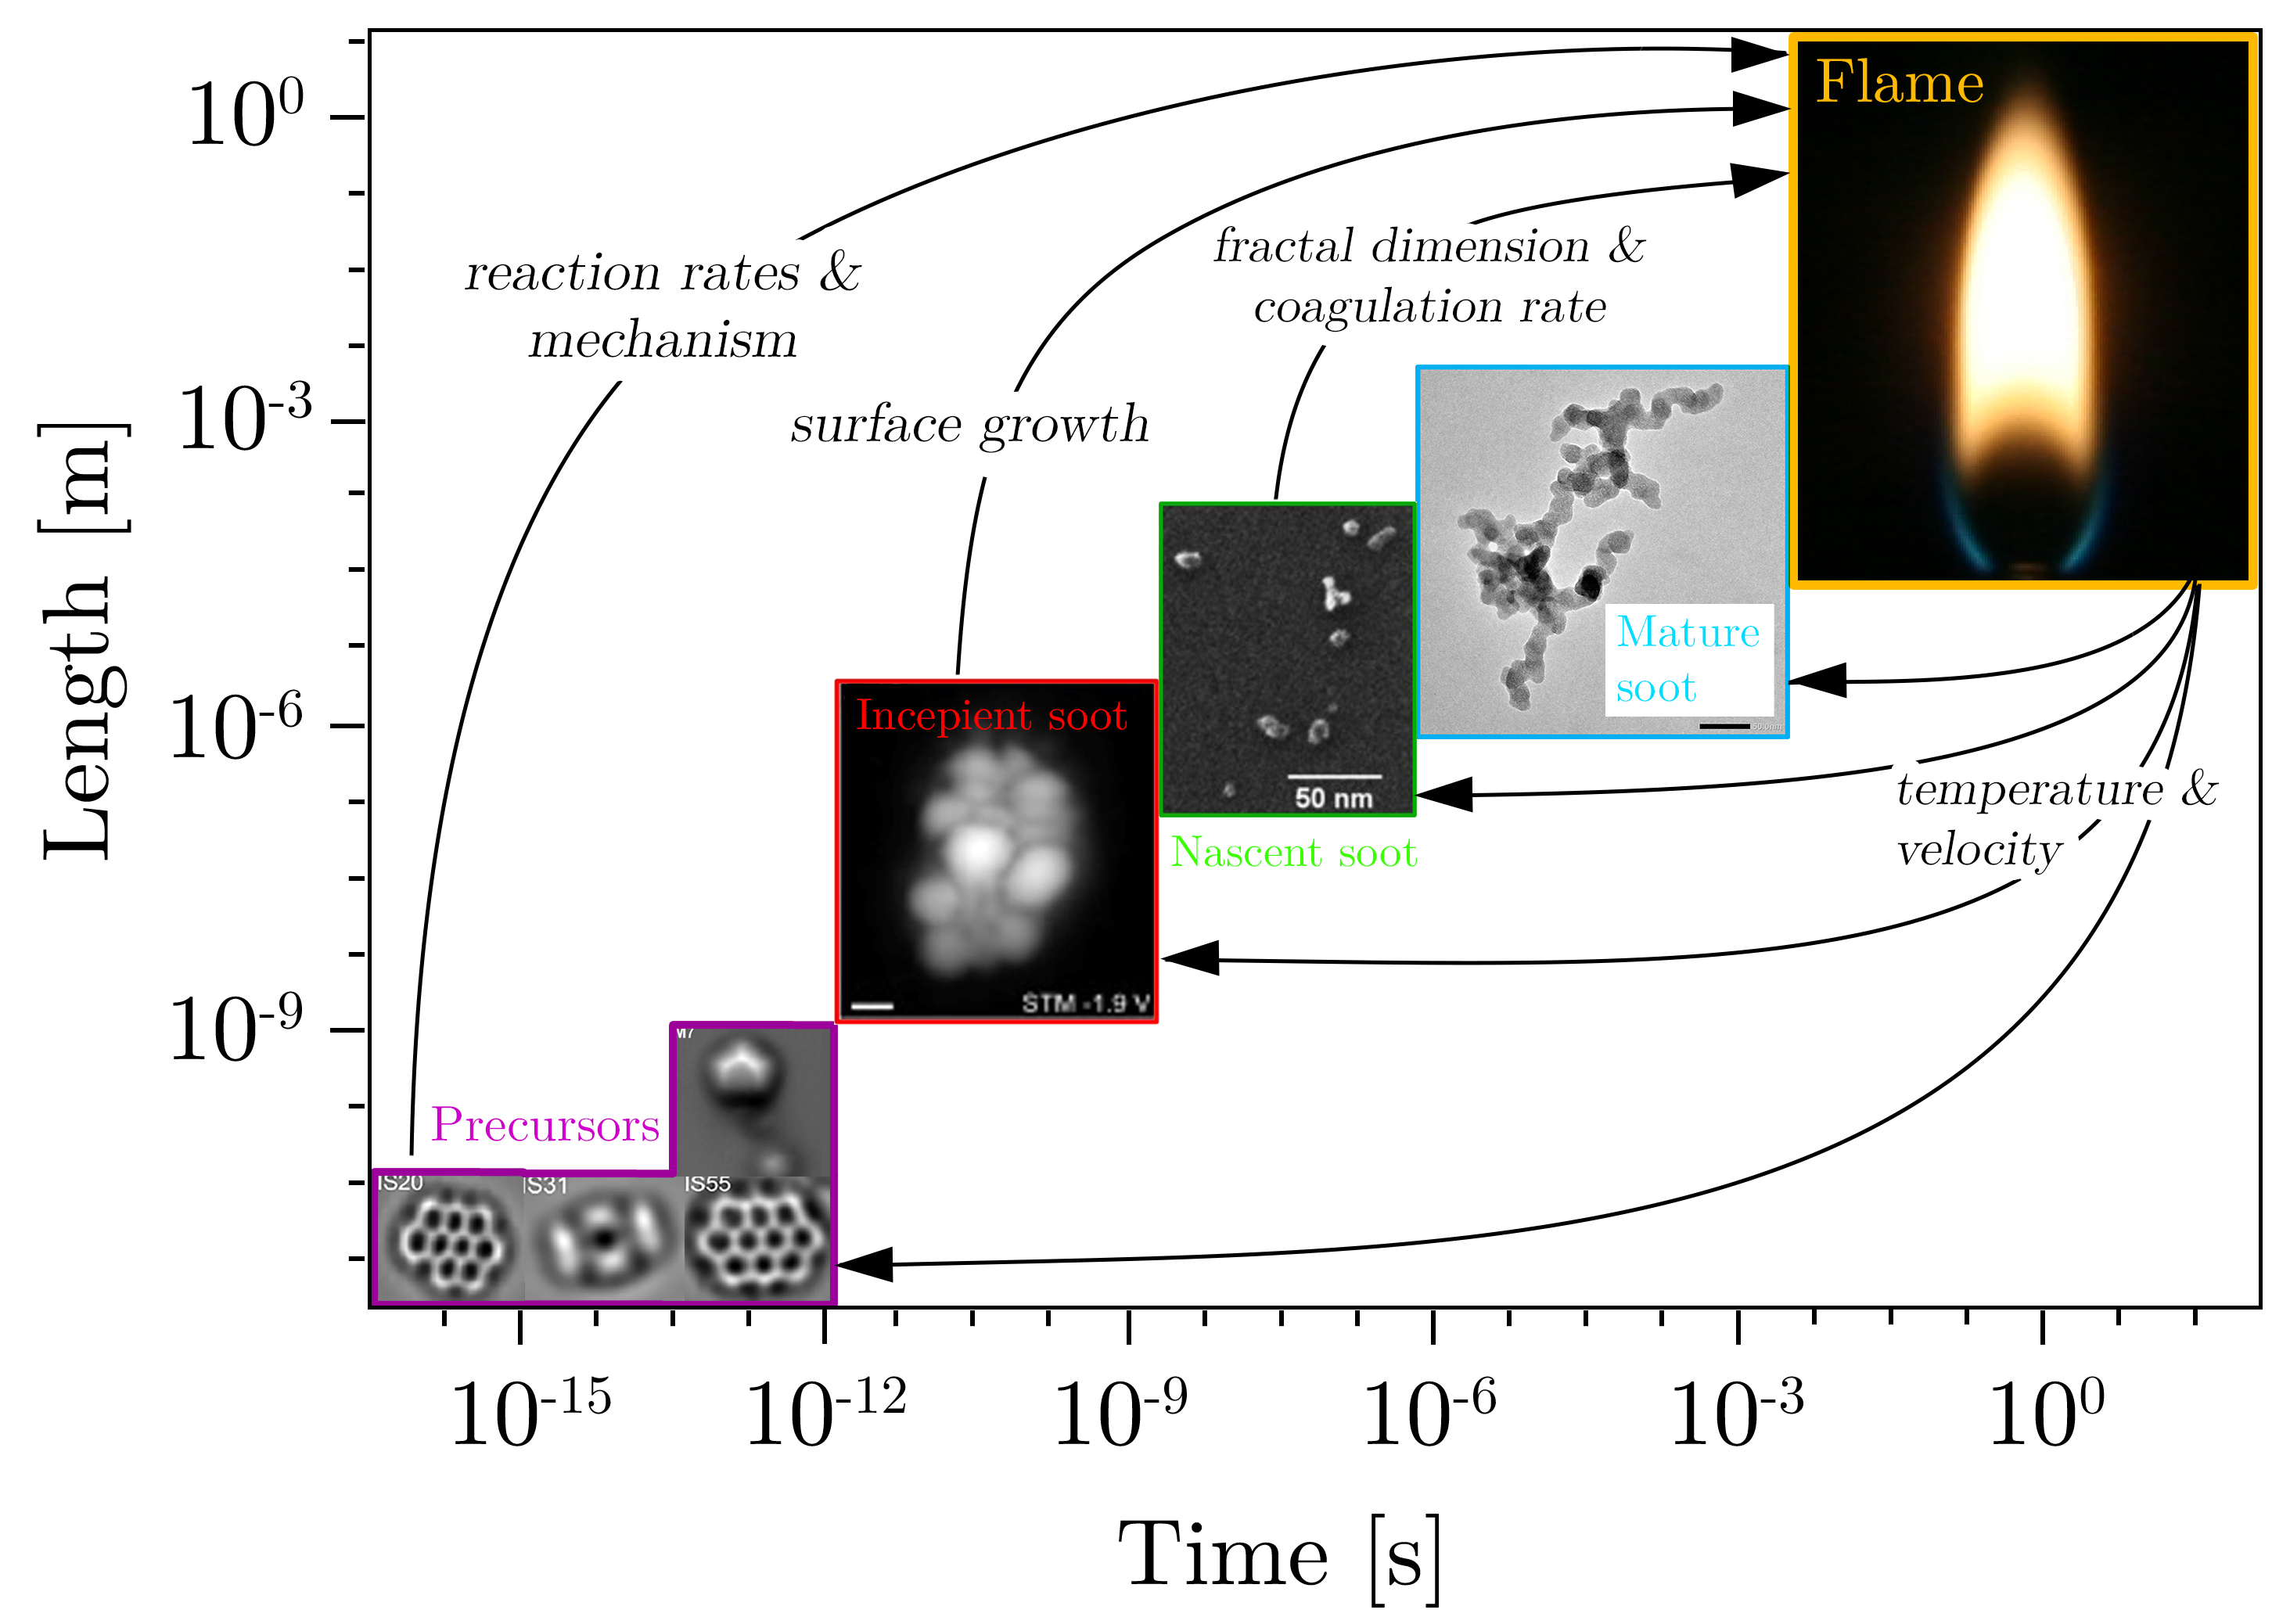
\includegraphics[width=0.7\textwidth]{Figures/Introduction/tlscales.jpg}};
		\draw (-2.45, -1.63) node[text=magenta] {\tiny{
				\citeColored{magenta}{commodo2019early}
		}};
		\draw (-1.99, -1.25) node[text=red] {\tiny{
				\citeColored{red}{schulz2019insights}
		}};
		\draw (-0.65, -0.7) node[text=green] {\tiny{
				\citeColored{green}{schenk2013imaging}
		}};
		\draw (0.39, -0.03) node[text=cyan] {\tiny{
				\citeColored{cyan}{kholghy2021morphology}
		}};					
		\draw (2.3, 3.2) node[text=orange] {\footnotesize{
				\citeColored{orange}{johansson2017evolution}
		}};		
	\end{tikzpicture}
	\caption{The processes involved in soot formation span a wide range of time and length scales, including molecular reactions between precursors, surface growth, coagulation of incipient and nascent soot particles, and their maturation, which is governed by the temperature-time history determined by flame velocity and temperature.}
	\label{fig:sootscales}
\end{figure}



Controlling CB yield, structure, morphology, and composition is essential for producing specific grades of CB tailored to target applications in both conventional (e.g., furnace process~\citep{dames2023plasma}) and emerging production methods~\citep{li2017experimental, fulcheri2023energy, patlolla2023review}. However, the influence of process parameters such as feedstock composition, pressure, and temperature–time history on CB properties remains incompletely understood due to the complexity of gas-phase chemistry and the intricate nature of CB formation (as discussed in the following sections). This underscores the need for robust computational models to predict yield, particle structure, and composition under varying process conditions, and to support the mitigation of soot emissions from combustion systems.


\textit{"Soot"} and \textit{"Carbon Black"} are distinct materials in terms of chemical properties and synthesis processes~\cite{watson2001carbon}. While, soot usually refers to unwanted particulate matter formed during incomplete combustion with variable organic content and a large variation in carbon to hydrogen (C/H) ratio~\citep{watson2001carbon}, CB is commercially produced under highly controlled partial combustion or thermal decomposition of hydrocarbons. However, soot particles generated under controlled laboratory conditions can have similar structure and composition to CB. Mature soot formed in methane and ethylene premixed flames can reach elemental C/H$\approx$20~\cite{russo2015dehydrogenation}, which is close to C/H of CB. The comparison of Transmission Electron Microscopy (TEM) images of industrially produced CB~\citep{singh2018nanostructure} with soot sampled from diesel fuel~\citep{vander2007hrtem, lapuerta2017morphological} indicates similarities in their morphology and structure. Hereafter, soot will be used to collectively refer to carbonaceous nanoparticles produced during combustion/pyrolysis processes.


Soot inception is believed to begin with the formation of Polycyclic Aromatic Hydrocarbons (PAHs) in the gas phase and followed by their transition into incipient particles. Soot inception remains poorly understood at the level of pathways and elementary reactions~\citep{Wang2011}. This lack of understanding stems primarily from uncertainties in PAH chemistry and the kinetics of PAH growth into soot particles, a process that is highly reversible and thus sensitive to local conditions such as temperature, pressure, and the concentrations of intermediate species~\citep{Wang2011}.


The classic description of soot inception relies on PAH dimerization where collision of two PAH molecules (monomers in this context) forms a dimer held together by van der Waals forces (vdW)~\citep{frenklach1991detailed}. The dimerization is an irreversible process with an efficiency that accounts for the reversibility or dissociation of dimers. The theory postulates that PAH growth continues by sequential addition of monomers forming stacks of dimers, trimers, tetramers, and so on to reach a certain mass threshold that marks the emergence of incipient soot~\citep{frenklach1991detailed}, but for practical purposes, a dimer is usually considered as incipient soot. Here, we call this model \textit{Irreversible Dimerization}. 
Irreversible Dimerization has been used to predict soot formation in burner-stabilized premixed~\citep{salenbauch2015modeling, desgroux2017comparative}, counterflow diffusion flames~\citep{wang2015soot, xu2021experimental}, and coflow diffusion flames~\citep{kholghy2016core, veshkini2016understanding}. A collision efficiency factor ranging between $10^{-6}$ to 1 is also employed to adjust the inception flux and PAH adsorption rates to achieve desired soot mass and size distribution. PAHs of moderate sizes, such as pyrene (4 rings) to coronene (7 rings), are typically considered as the starting point of inception due to their thermodynamic stability, which justifies the irreversibility at high temperatures~\citep{frenklach1991detailed}. However, the theoretical calculations~\citep{miller1985calculations} and experiments~\citep{sabbah2010exploring} indicated that PAH dimerization is highly reversible in flame conditions. The inception flux of irreversible dimerization is mainly controlled by PAH concentration due to its weak temperature dependence, so it produces new particles at low temperatures (even below 500 K)~\citep{naseri2022simulating} despite experimental evidence for termination of inception below 1200 K~\citep{sanchez2012polycyclic, cho2016synthesis}. 



\citet{kholghy2019role} emphasized the necessity of chemical bond formation following physical PAH clustering for accurate prediction of volume fraction, primary particle diameter, and particle size distribution (PSD) in ethylene coflow diffusion flames. \citet{kholghy2018reactive} proposed the \textit{Reactive Dimerization} model, which begins with the reversible collision of PAHs to form physical dimers stabilized by van der Waals forces. These dimers are subsequently graphitized and form chemically bonded dimers that act as incipient soot, which then grow via coagulation and surface reactions. They also conducted a systematic analysis of the contributions of different PAHs and concluded that one- and two-ring aromatics account for nearly all of the inception flux in so-called \textit{sooting flames}~\citep{desgroux2017comparative}. 

However, \citet{frenklach2020mechanism} argued that an inception model initiated by a highly reversible step, such as that in Reactive Dimerization~\citep{kholghy2018reactive}, cannot generate a sufficient particle flux to match measurements in the benchmark burner-stabilized stagnation flame~\citep{abid2009quantitative}. Instead, they proposed the H-abstraction-$\mathrm{C_2H_2}$/Carbon-addition~\citep{frenklach1991detailed, appel2000kinetic} (HACA)-driven mechanism where addition of a monomer molecule to its radical activated by hydrogen abstraction forms a stable dimer via an E-Bridge bond formation, and this sequential process continues to form trimers, tetramers, and larger PAH clusters. %\citet{blanquart2009joint} proposed a two-step irreversible inception model where self collision of PAHs with specified efficiencies results in the formation of dimers that collide and subsequently coalesce into an incipient soot.

The gas-phase chemistry of aromatics can be extended to account for chemical growth of incipient soot via surface reactions~\citep{frenklach2002reaction}. This hypothesis, known as “chemical similarity”, postulates that the reactions occurring on the soot surface are similar to those involving large molecules of PAHs in the gas phase. It also provides a means to describe the rates of surface growth and particle oxidation in
terms of elementary chemical reactions. In other words, it is assumed that the surface of soot particles is made up of lateral faces of large PAHs covered with C-H bonds.
This is the basis for HACA mechanism~\citep{frenklach1991detailed, appel2000kinetic} that assumes the soot surface consists of hydrogenated sites with a predefined density. Mass growth on the soot surface requires H-abstraction to form a radical
site, followed by acetylene attack similar to the growth of PAH molecules in the gas phase. The reactivity of these sites changes with time and temperature~\citep{woods1991soot, dasch1985decay}, described as soot aging. For modeling purposes, a temperature-dependent surface reactivity, usually represented by $\alpha$, was introduced to account for the depletion of reactive sites with soot maturity. \citet{appel2000kinetic} showed $\alpha$ changes with temperature and particle size in laminar premixed flames.


Adsorption of PAHs on the surface of soot particles is also a viable growth mechanism~\citep{frenklach1991detailed}, more specifically called physisorption or chemisorption depending on the mechanisms driving the adsorption process~\citep{michelsen2020review}. There is still debate over the stability of adsorbed PAH molecules on soot surface~\citep{obolensky2007interplay}. Following the hypothesis that PAHs are building blocks of soot particles, a mechanism similar to inception is often used to describe PAH-soot growth.


In typical soot formation processes, such as those occurring in flames and reactors, inception and surface growth are active for only a relatively short duration compared to the total residence time of soot particles. Subsequently, due to high particle concentrations, coagulation becomes the dominant mechanism, rapidly leading to the development of both a Self-Preserving Size Distribution (SPSD)~\citep{lai1972self} and an asymptotic fractal-like structure~\citep{mountain1986simulation, Goudeli2016}.
The collision frequency of agglomerates depends on their evolving fractal-like morphology, with polydisperse agglomerates colliding more frequently than monodisperse ones. This enhancement reaches an asymptotic value of 35$\%$~\citep{Goudeli2016} in the free molecular regime or 82$\%$~\citep{kelesidis2021self} in the transition regime at SPSD, irrespective of primary particle polydispersity.

Particle morphology, governed by inception, surface growth, and agglomeration, can be precisely tracked using mesoscale simulations such as Discrete Element Modeling (DEM)~\citep{Kelesidis2017Flame} provided that the gas-to-particle mass flux through inception and surface growth is known a priori. However, these methods are computationally expensive, and integrating them with chemical kinetics in Computational Fluid Dynamics (CFD) frameworks is challenging~\citep{kelesidis2021perspective}. Consequently, their application is often limited to canonical scenarios where particle dynamics are solved independently of chemistry and flow dynamics, typically by populating the simulation domain with incipient particles and neglecting the removal or addition of gaseous species due to soot formation~\citep{Kelesidis2017} as it is difficult to have a particle dynamics modeled fully coupled with gas chemistry. 

As a computationally efficient alternative, particle dynamics can be tracked by Eulerian approaches such as the Method of Moments (MOM)~\citep{kazakov1998dynamic} or Monodisperse Population Balance Models (MPBM)~\citep{kruis1993simple}. Such models only track average particle properties and their accuracy can be limited if unrealistic assumptions such as approximating agglomerates as spheres are used. However, when inception and surface growth are short~\citep{Spicer2002} and high particle number concentrations are formed~\cite{Kelesidis2017}, they lead to rapid attainment of SPSD and agglomerates having asymptotic structure~\citep{Goudeli2016}. In this case, a MPBM or MOM can be assembled on a firm scientific basis with accuracy on par with DEM~\citep{Kelesidis2017Flame} and experimental data ~\citep{abid2008evolution, ma2013soot, camacho2015mobility}. Such models can be readily interfaced with CFD simulations~\citep{grohn2012fluid} without significant computational cost, making them ideal for three-dimensional and even turbulent flame simulations.

The main difficulty of MOM is the closure of transport equations terms rising from expressing inception, surface growth and coagulation source terms based on the tracked moments~\citep{frenklach2002method}. In contrast, MPBMs do not have the closure problem and calculate average particle properties by tracking their total concentration, mass \citep{kruis1993simple} and area~\citep{tsantilis2004soft, lindstedt1994simplified}. 

Sectional Population Balance Models (SPBMs) are similar to MPBMs but capable of tracking agglomerate and primary PSDs~\citep{Xiong1993}. SPBMs can solve one, two, or three equations per section, with their capabilities depending on the number of equations solved: single-equation models track basic properties like total mass or number concentration~\citep{gelbard1980sectional}, two-equation models capture additional details such as surface area or primary particle number~\citep{park2004novel}, and three-equation models enable detailed tracking of complex properties like composition or morphology~\citep{kholghy2016core}. Coupled with relations for fractal-like structure~\citep{matsoukas1991dynamics} and collision frequency~\citep{fuchs1964mechanics}, SPBMs can accurately model particle size distribution, morphology, and composition. However, their computational cost rises exponentially with the number of sections~\citep{xiong1993formation} and tracked properties~\citep{kholghy2016core}.

 
SPBMs are gaining attention, due to the recent increase in computational resources, for simulating laminar and turbulent benchmark flames in two-dimensional domains, even with moderately large chemical mechanisms. For example, the CoFlame solver~\citep{eaves2016coflame}, designed to simulate laminar diffusion flames in axisymmetric domains using a SPBM, has been employed in numerous studies, demonstrating its ability to accurately capture soot morphological properties~\citep{dworkin2011application, liu2015numerical}. The CRECK group developed a sectional approach in which discrete size bins are embedded in the kinetic mechanism as lumped pseudo-species (BINs), covering the mass range from $\mathrm{C_{20}}$ PAHs to the largest agglomerates ($\mathrm{C_{10^7}}$)~\citep{cuoci2015opensmoke++, cuoci2013computational}. This hybrid soot-gas mechanism, available in standard Chemkin file format, has been validated against a wide range of flame and reactor configurations~\cite{ramalli2023automatic}. However, portability and flexibility remain major challenges of this approach. The base gas-phase chemistry (excluding BINs) cannot be readily replaced with other mechanisms, which is important given the large uncertainty in the prediction of even small hydrocarbons (as discussed in Section~\ref{sec:uncergaschem}). In addition, the large size of the mechanism comprising 709 species and 109500 reactions~\citep{nobili2022modeling} poses a significant computational burden, particularly in parametric studies.


Here, we develop a computational package, called Omnisoot, which integrates Cantera~\citep{cantera} as a chemistry solver to simulate soot formation in reduced-order dimensions. The package provides a versatile soot model that can be coupled with all reaction mechanisms. Both particle dynamics models (MPBM and SPBM) are coupled with various soot inception and surface growth models,  offering flexibility to study soot formation alongside gas phase chemistry. This package facilitates fundamental investigations of soot formation, including pathway analysis, reaction mechanism evaluation, and inception flux estimation, while also supporting process design and optimization of CB production in industrial reactors under diverse fuel compositions, temperatures, pressures, and residence times. The theoretical background and governing equations for sub-models of Omnisoot are detailed in subsequent sections, followed by validation against benchmark DEM simulations and verification of mass and energy conservation across all models. Finally, three use cases of Omnisoot were demonstrated by predicting gas chemistry, soot yield, morphology, and size distribution in shock tubes, flow reactors, and perfectly stirred reactors.





